\documentclass[../../main/main.tex]{subfiles}
\begin{document}
\section{Payoff Analysis}

In Nash Equilibrium, a given hand combination $(x, y)$ uniquely determines the bettor's payoff, since both players play pure strategies. We can better understand the strategy profile by examining payoffs for all hand combinations over the unit square $[0, 1]^2$ (see Figure \ref{fig:payoffs}). For comparison, the first and last plots show the payoffs in Fixed-Bet Continuous Poker with a fixed bet size $B=1$ and No-Limit Continuous Poker, respectively. We will explore the relationship between the three games in more detail in section \ref{sec:strategic_convergence}.

\begin{figure}[h!]
    \begin{adjustwidth}{-1in}{-1in}
        % \vspace{-3cm} % Move the figure up into the top margin
        \centering
        \begin{minipage}{0.4\textwidth}
            \centering
            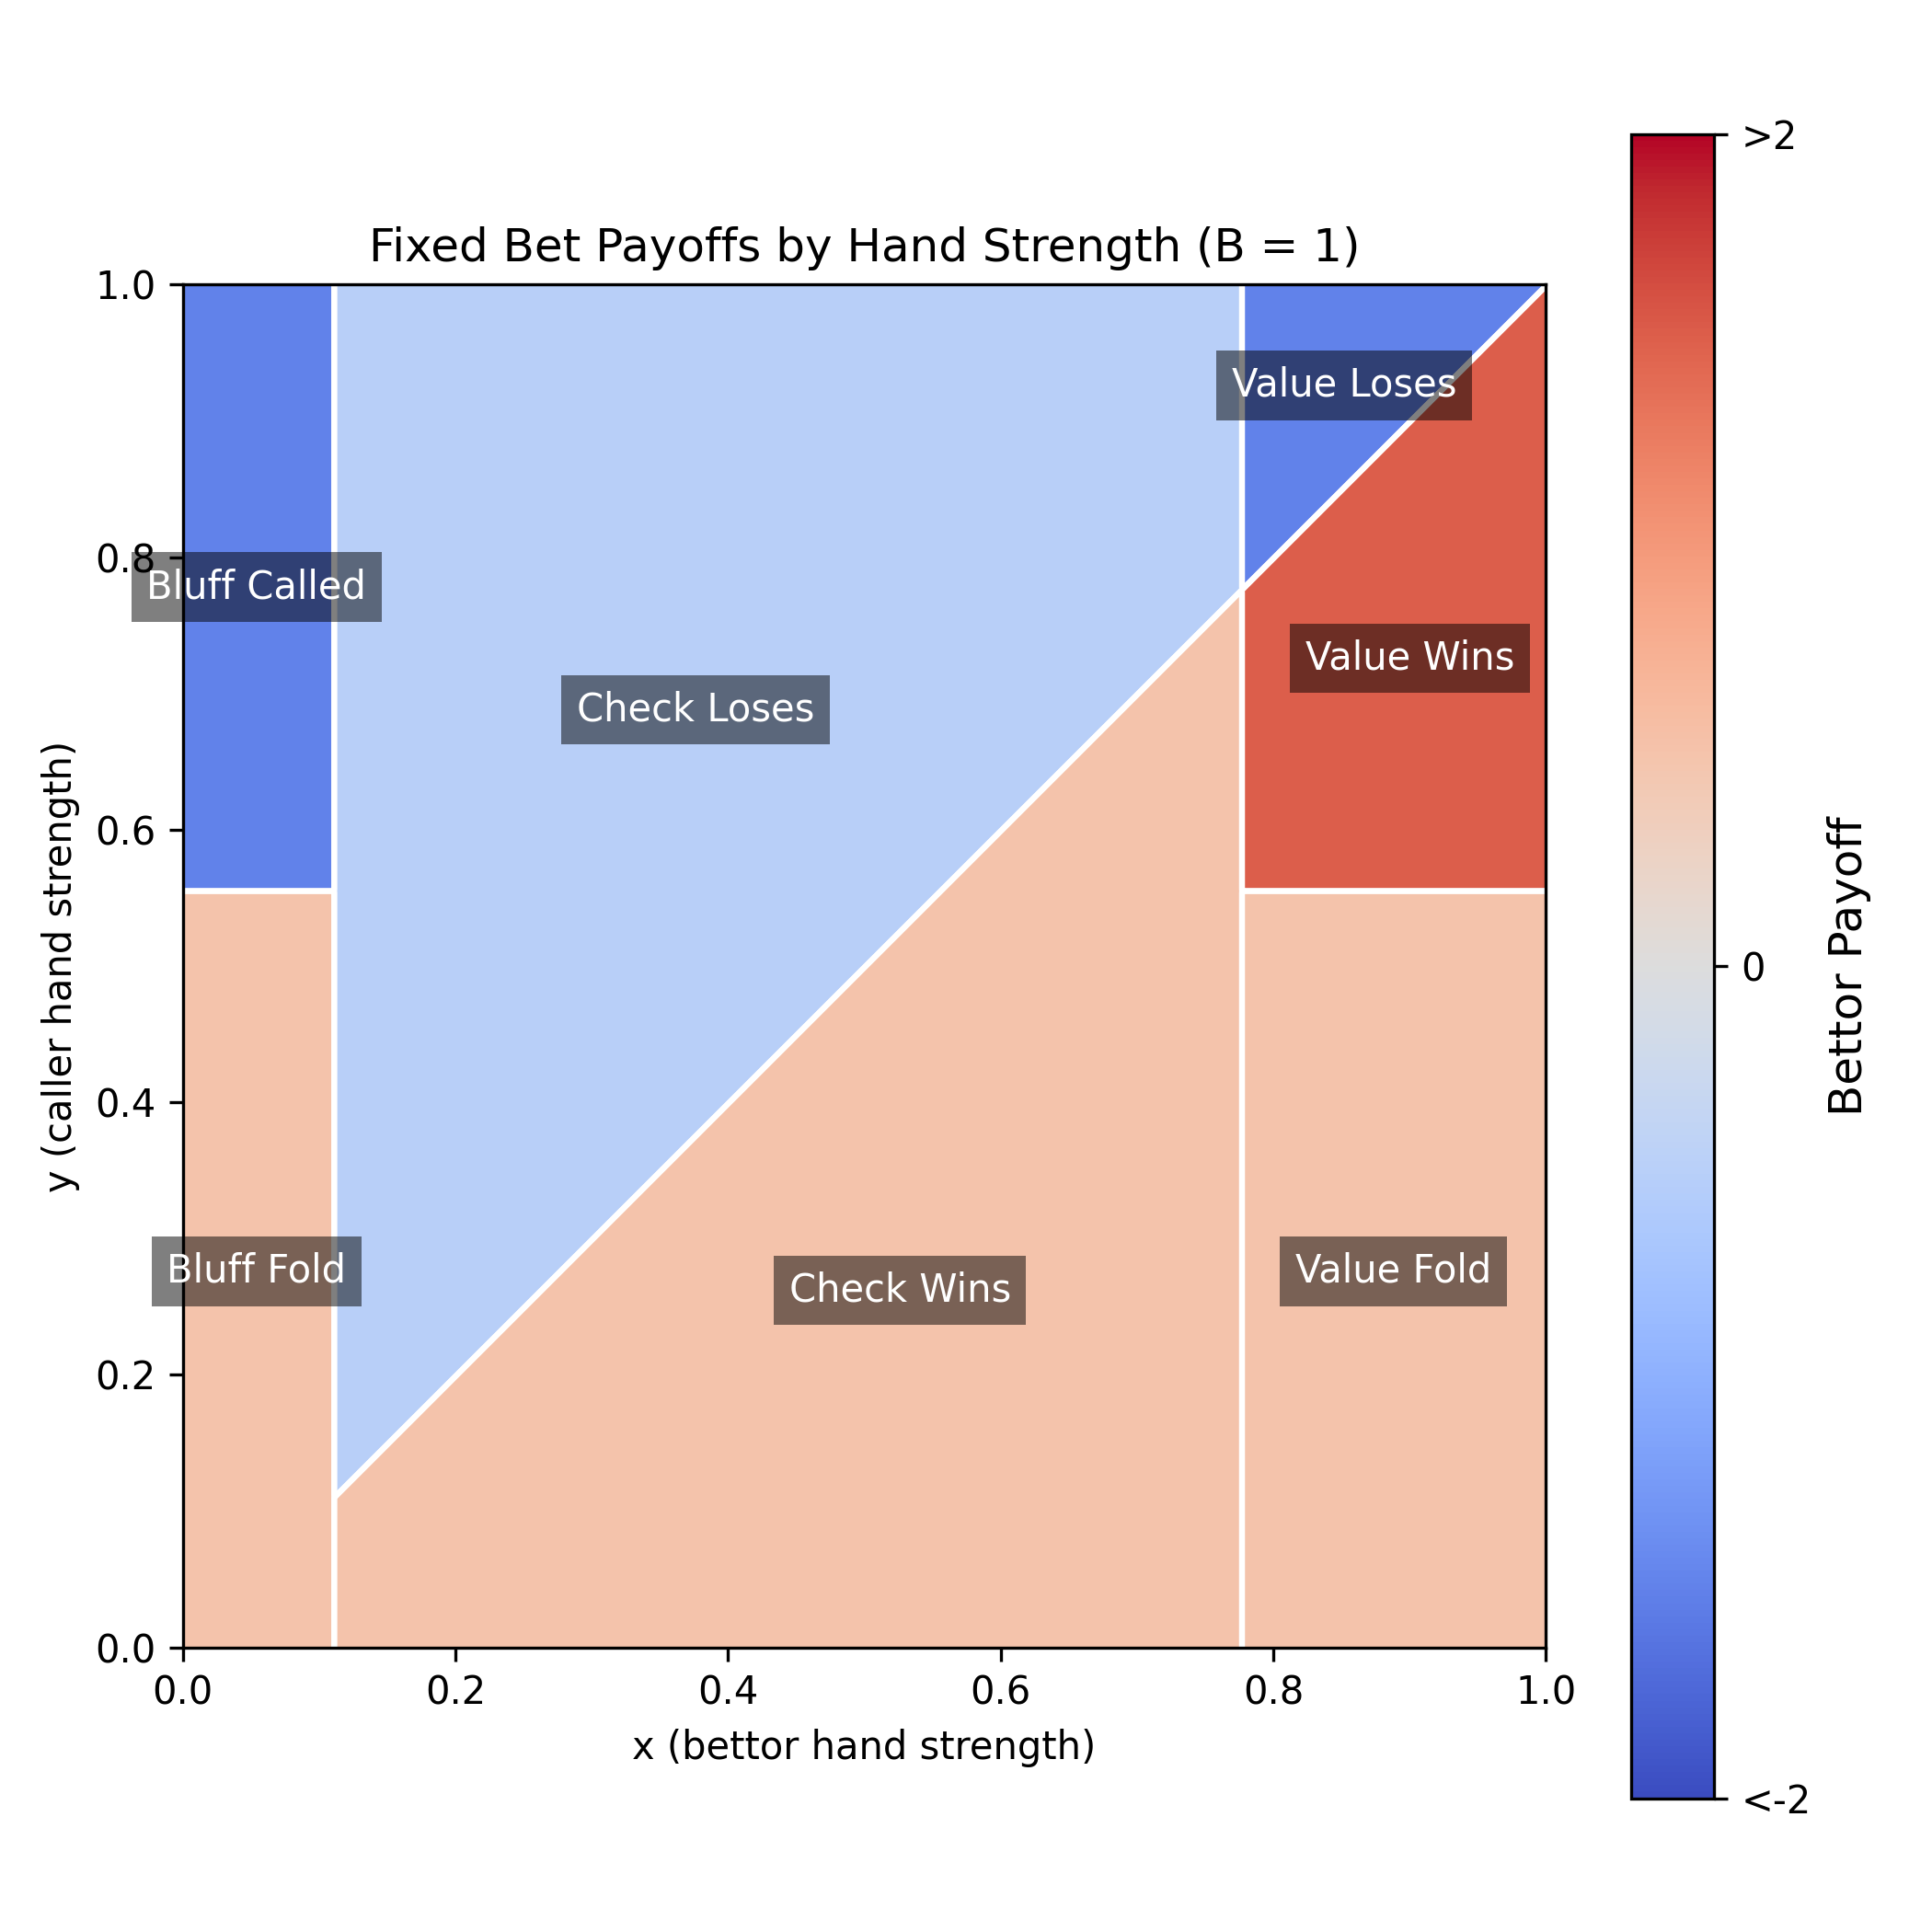
\includegraphics[width=\textwidth]{images/FixedBet_payoffs.png}
        \end{minipage}
        \hspace{0.02\textwidth}
        \begin{minipage}{0.4\textwidth}
            \centering
            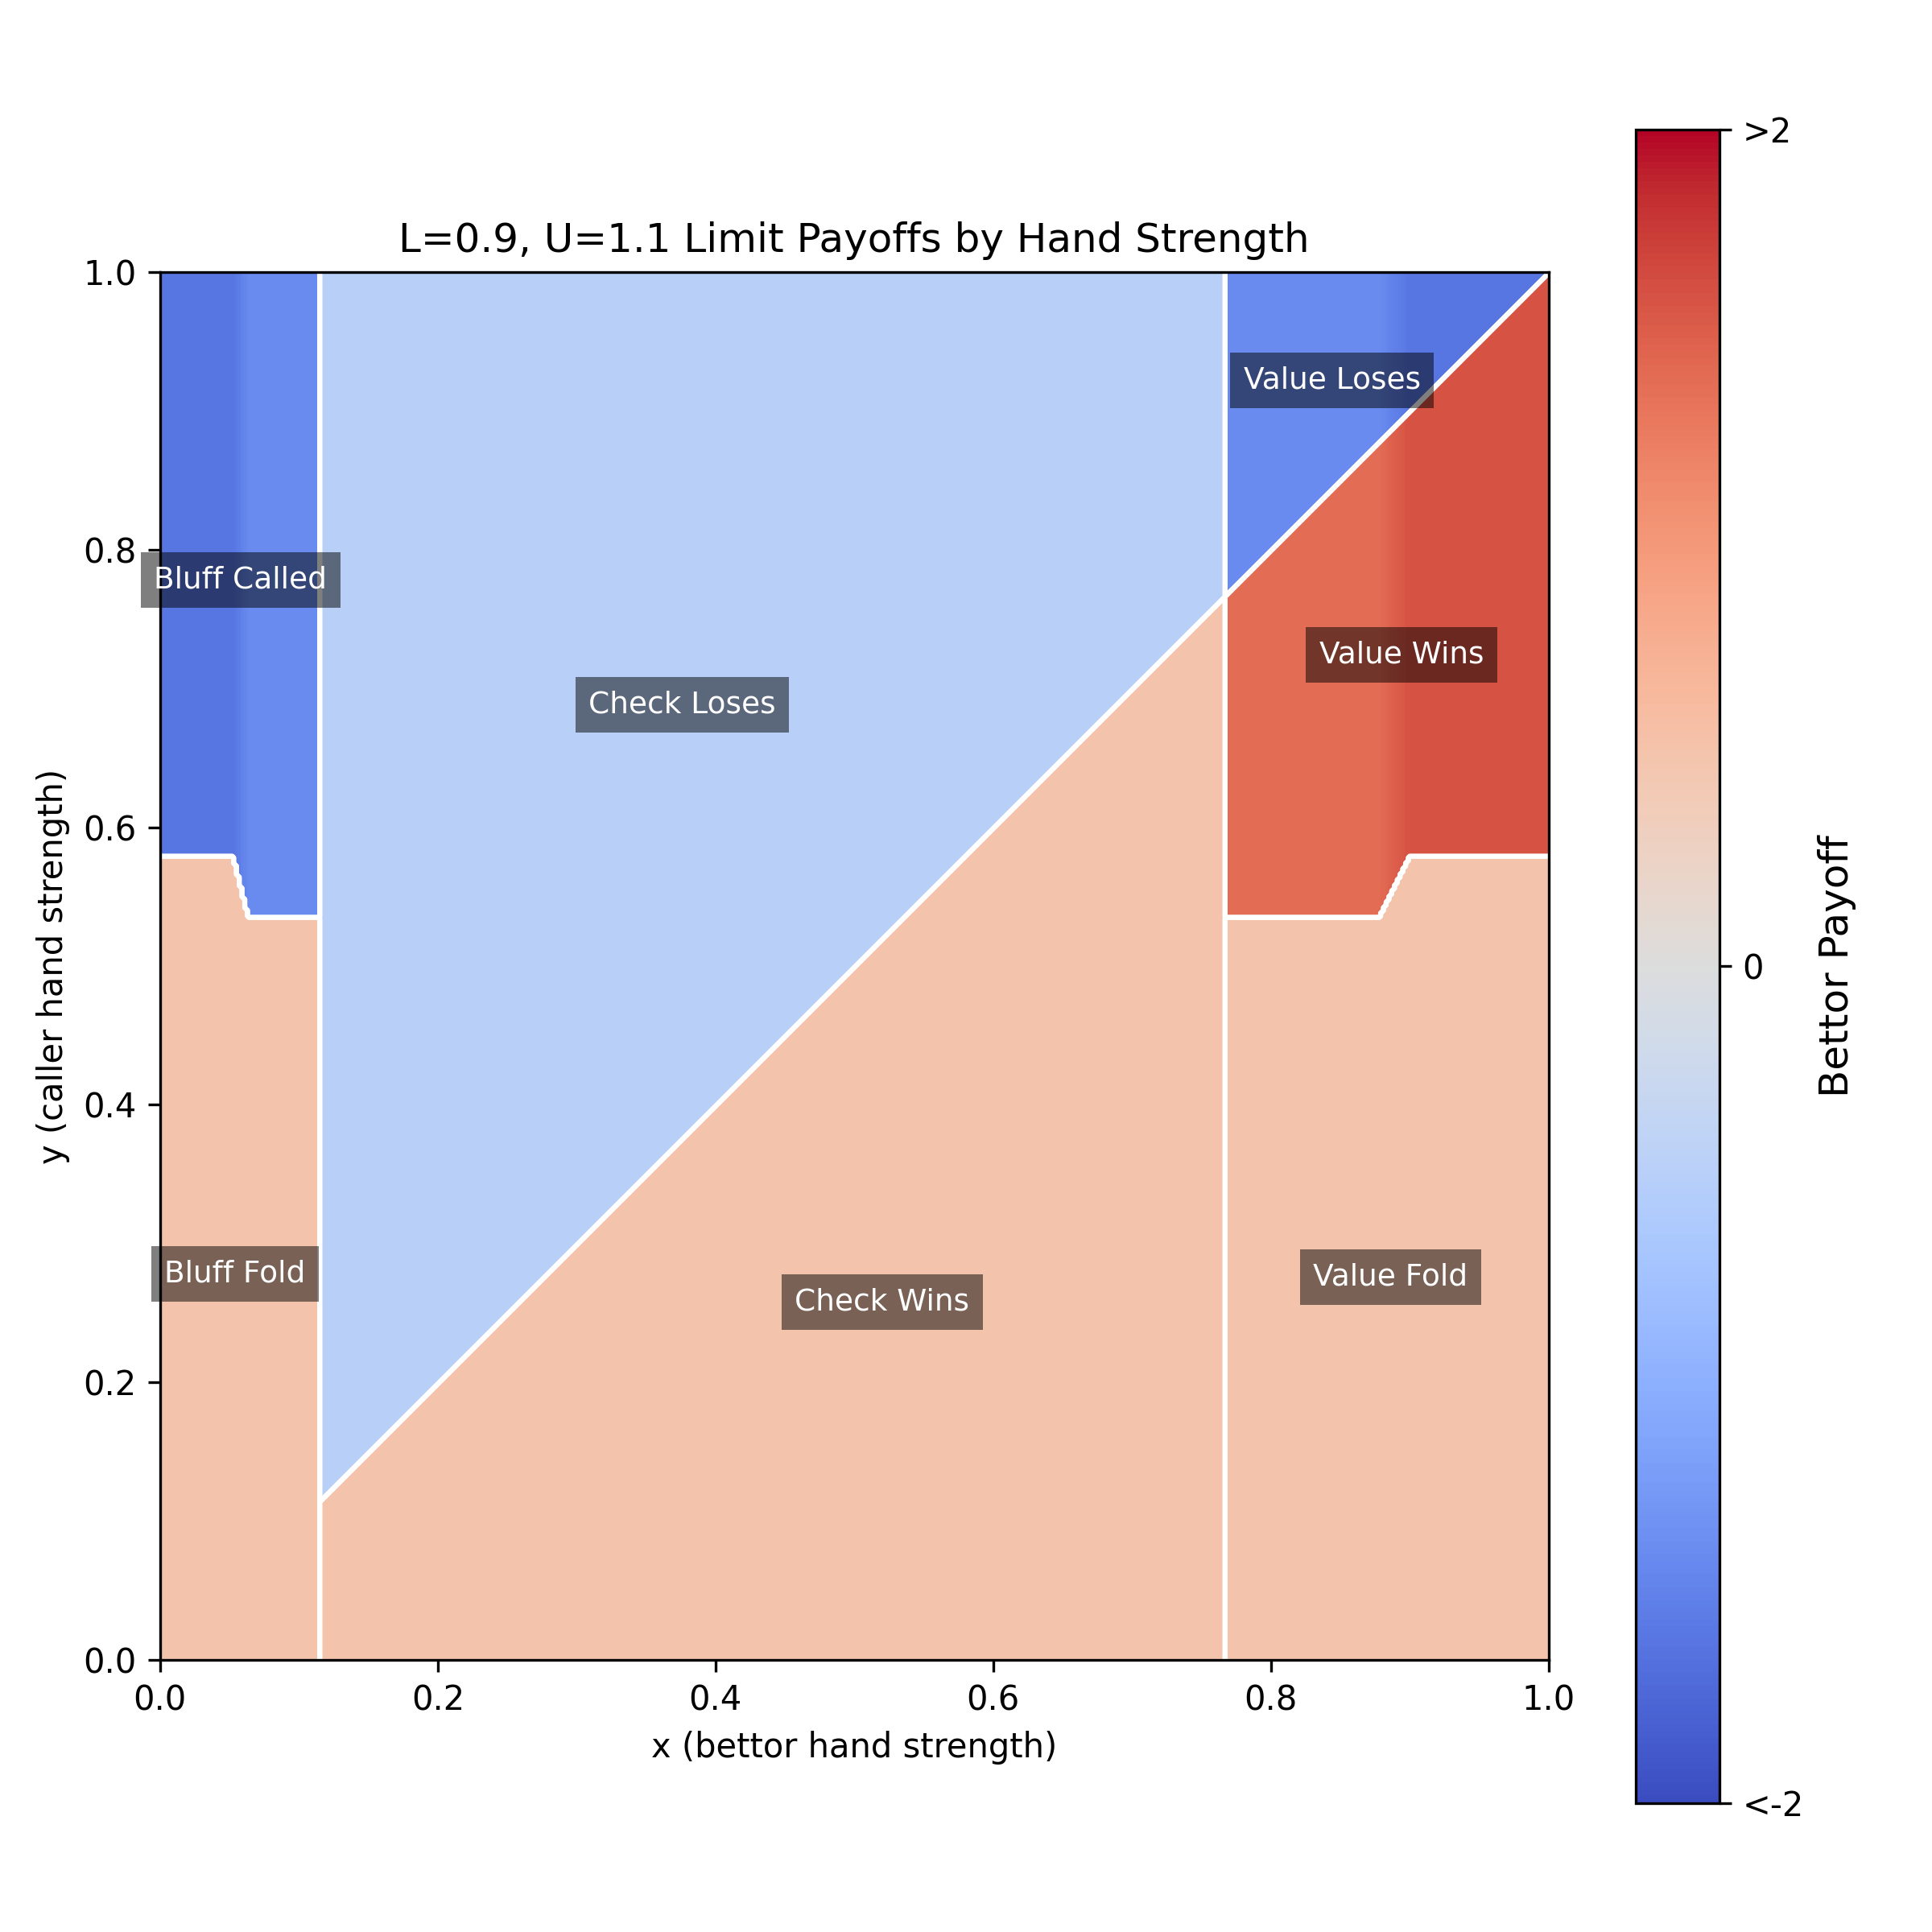
\includegraphics[width=\textwidth]{images/LU_payoffs_0.9_1.1.png}
        \end{minipage}
        \hspace{0.02\textwidth}
        \begin{minipage}{0.4\textwidth}
            \centering
            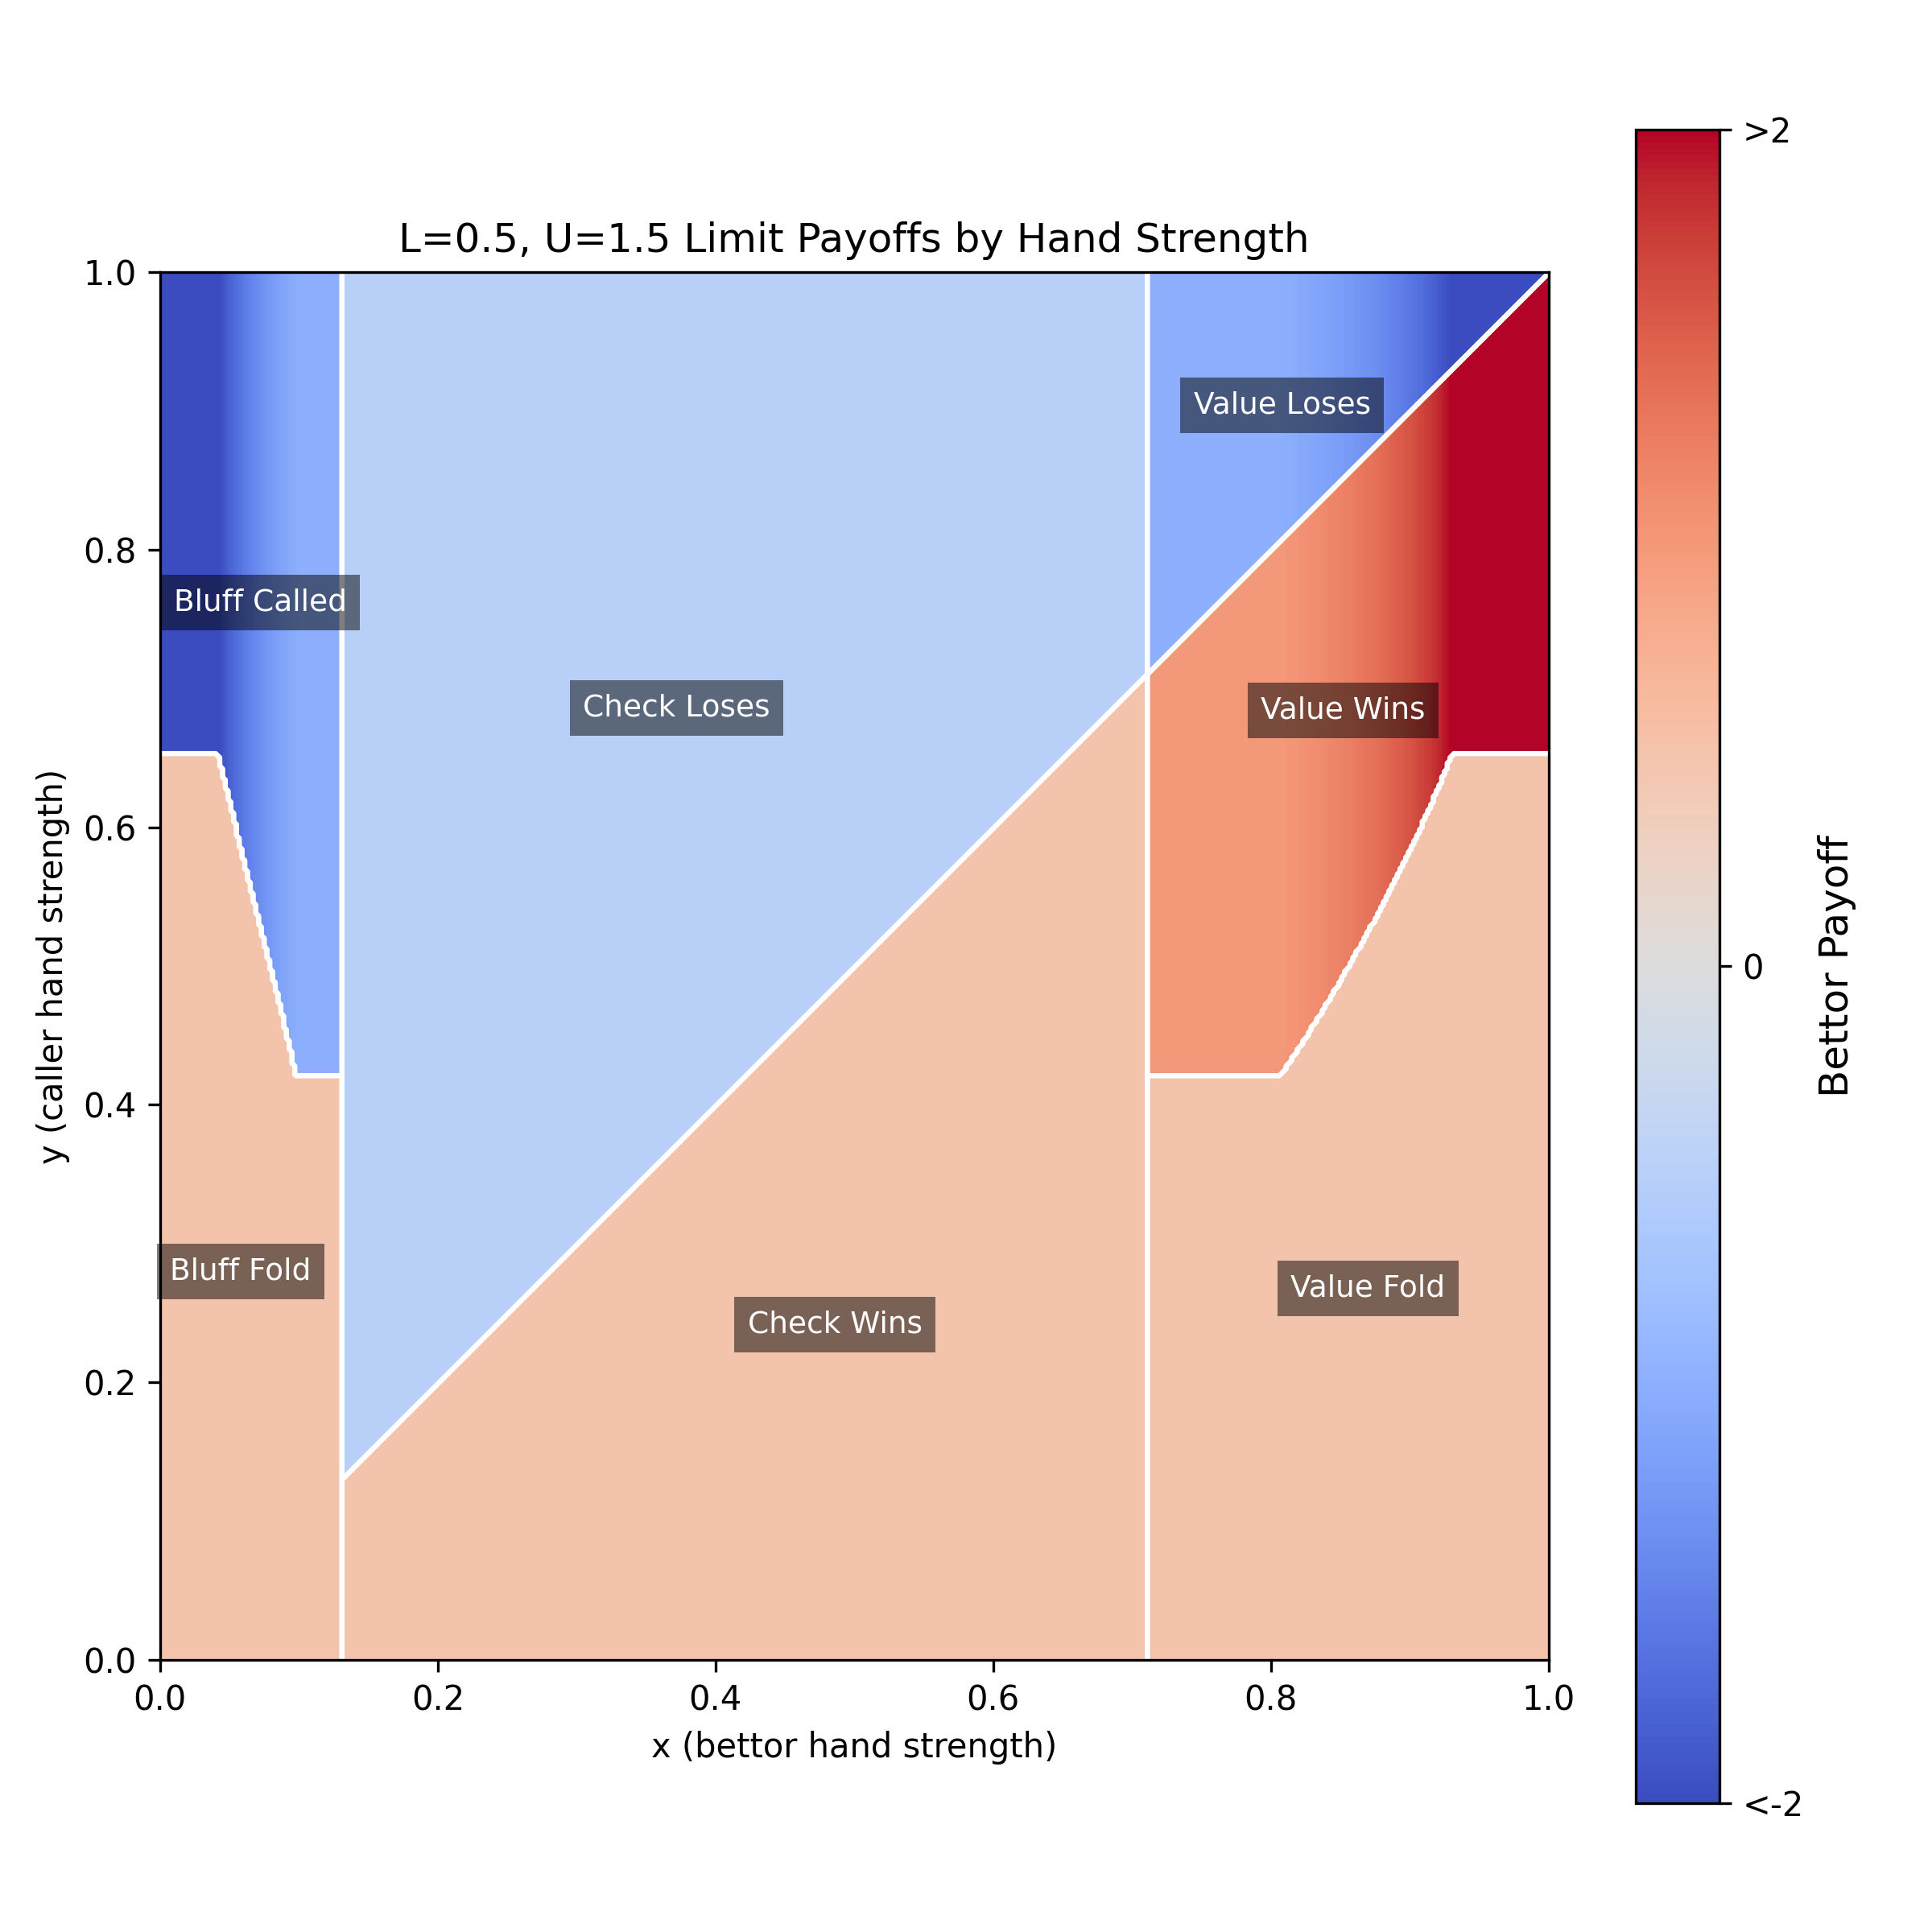
\includegraphics[width=\textwidth]{images/LU_payoffs_0.5_1.5.png}
        \end{minipage}
        \vspace{-0.5cm}\\ % Reduced vertical space
        \begin{minipage}{0.4\textwidth}
            \centering
            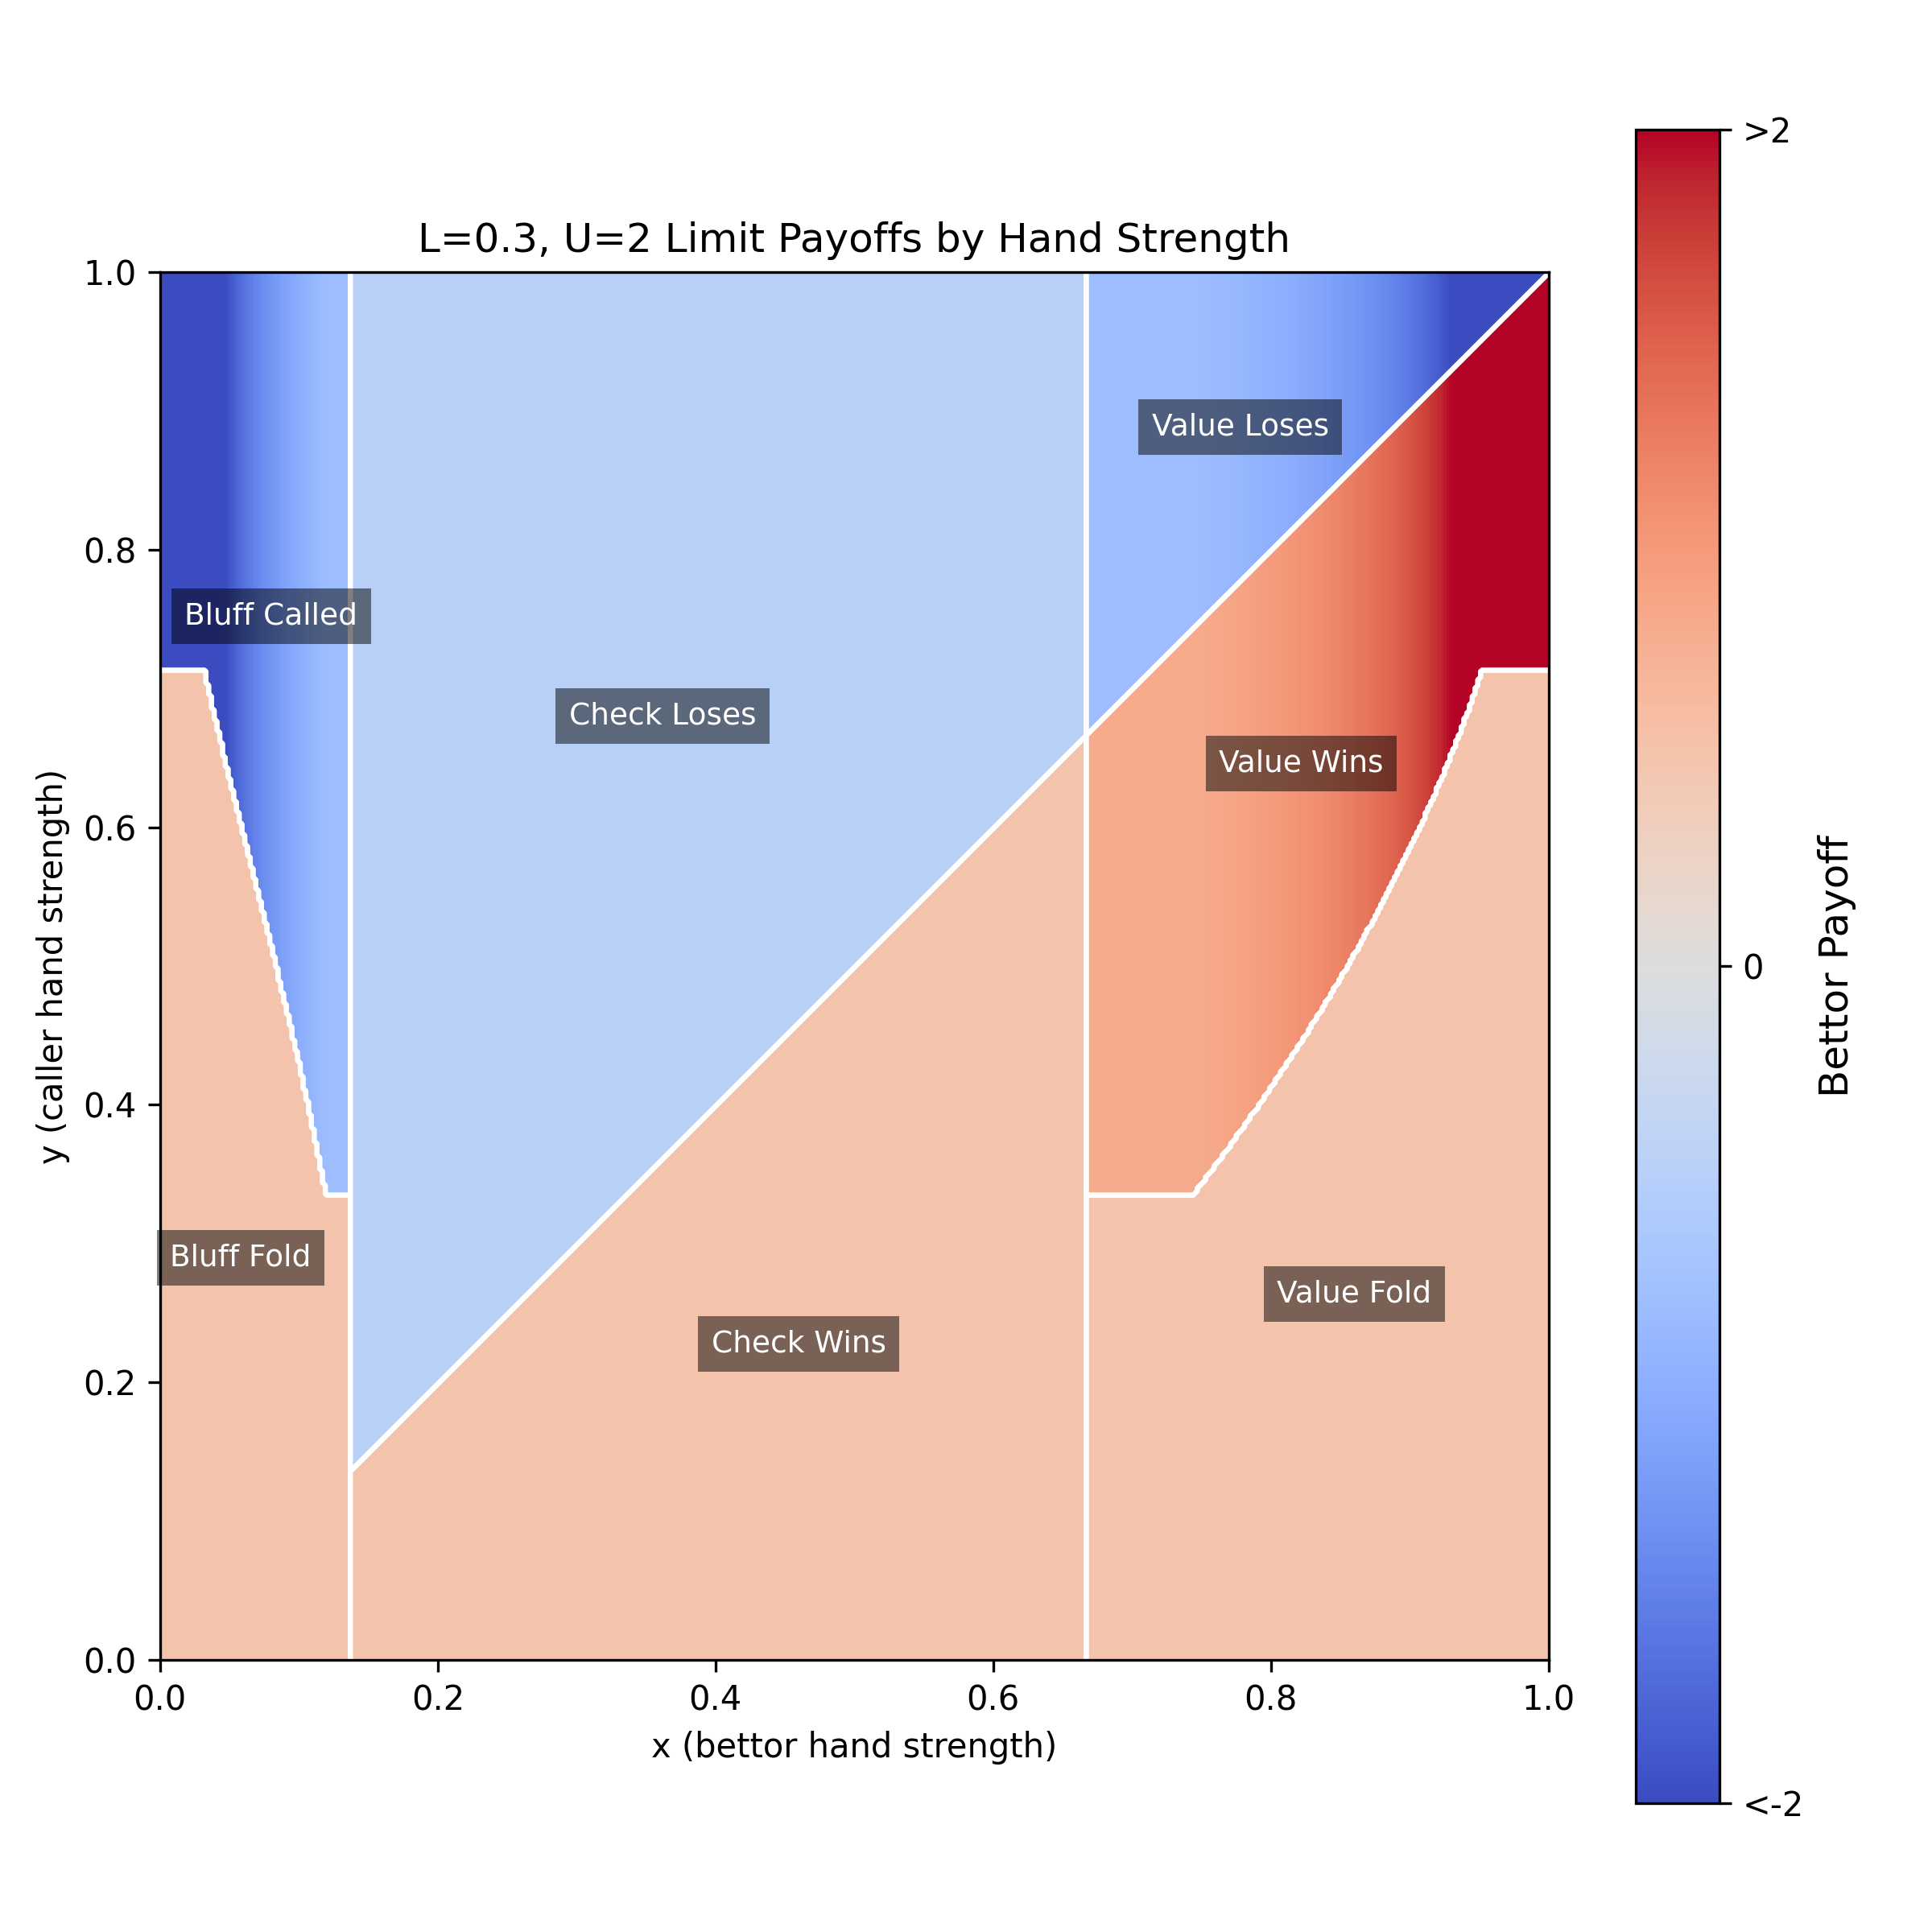
\includegraphics[width=\textwidth]{images/LU_payoffs_0.3_2.png}
        \end{minipage}
        \hspace{0.02\textwidth}
        \begin{minipage}{0.4\textwidth}
            \centering
            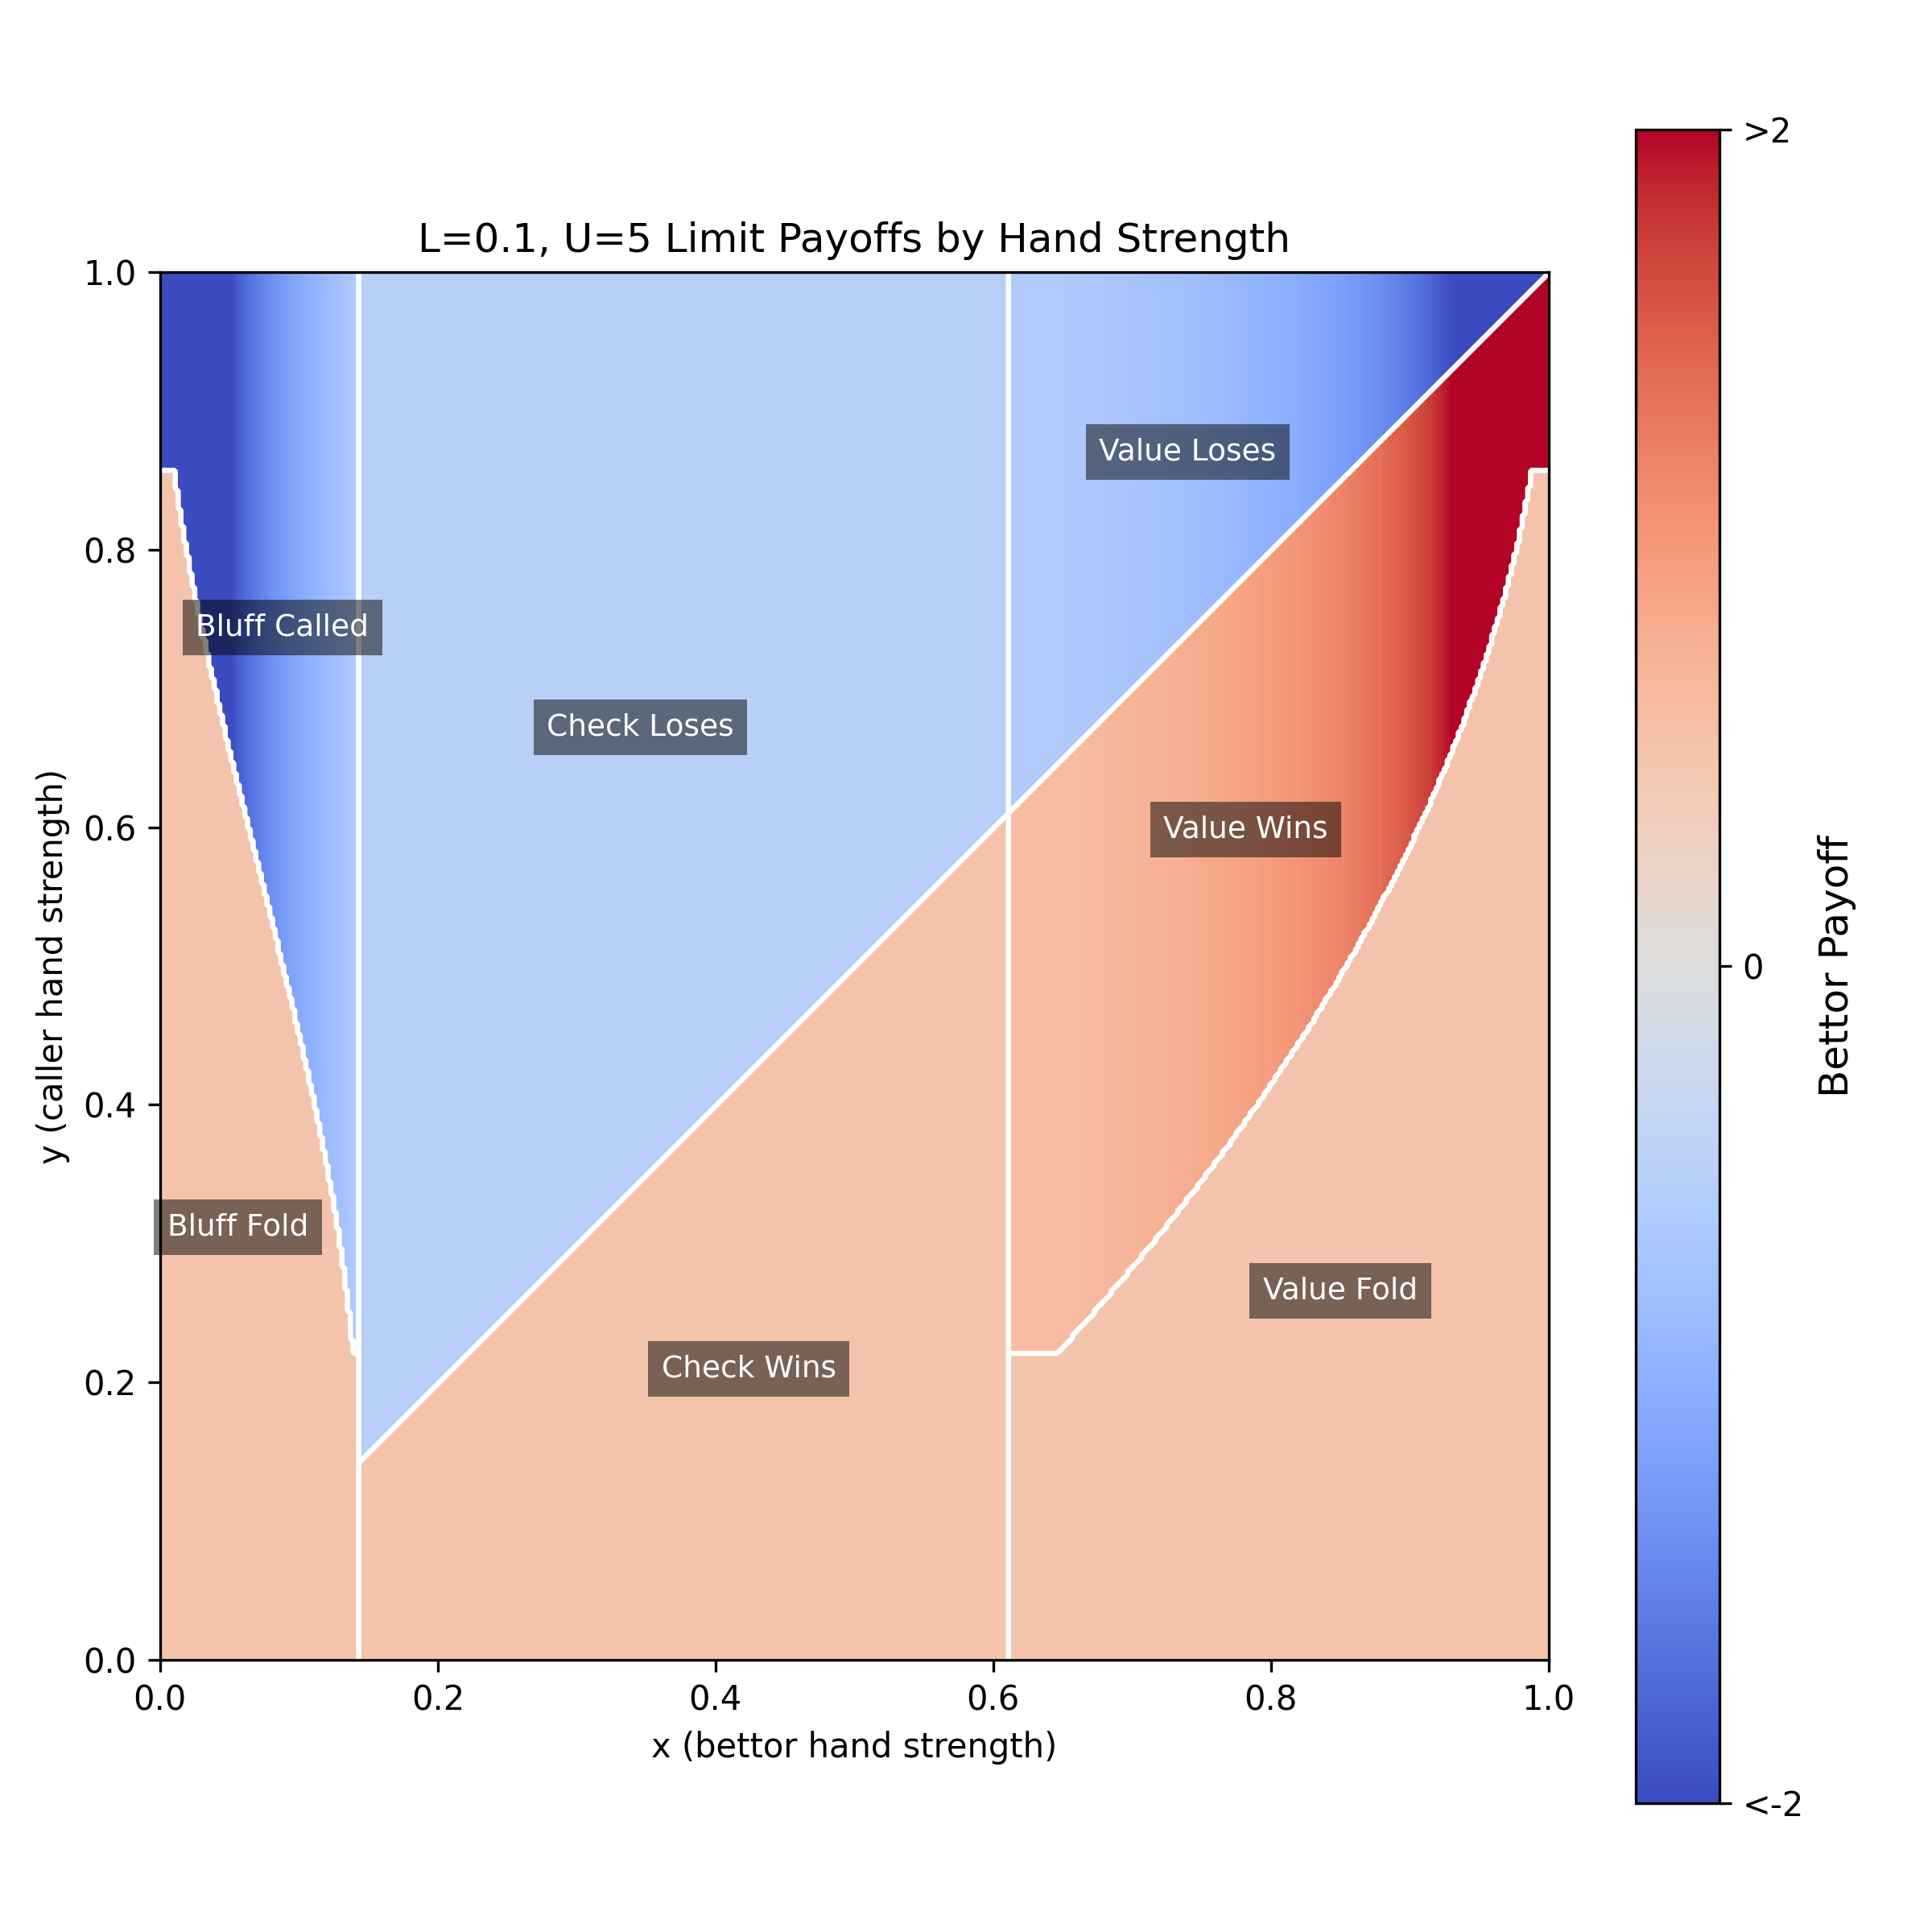
\includegraphics[width=\textwidth]{images/LU_payoffs_0.1_5.png}
        \end{minipage}
        \hspace{0.02\textwidth}
        \begin{minipage}{0.4\textwidth}
            \centering
            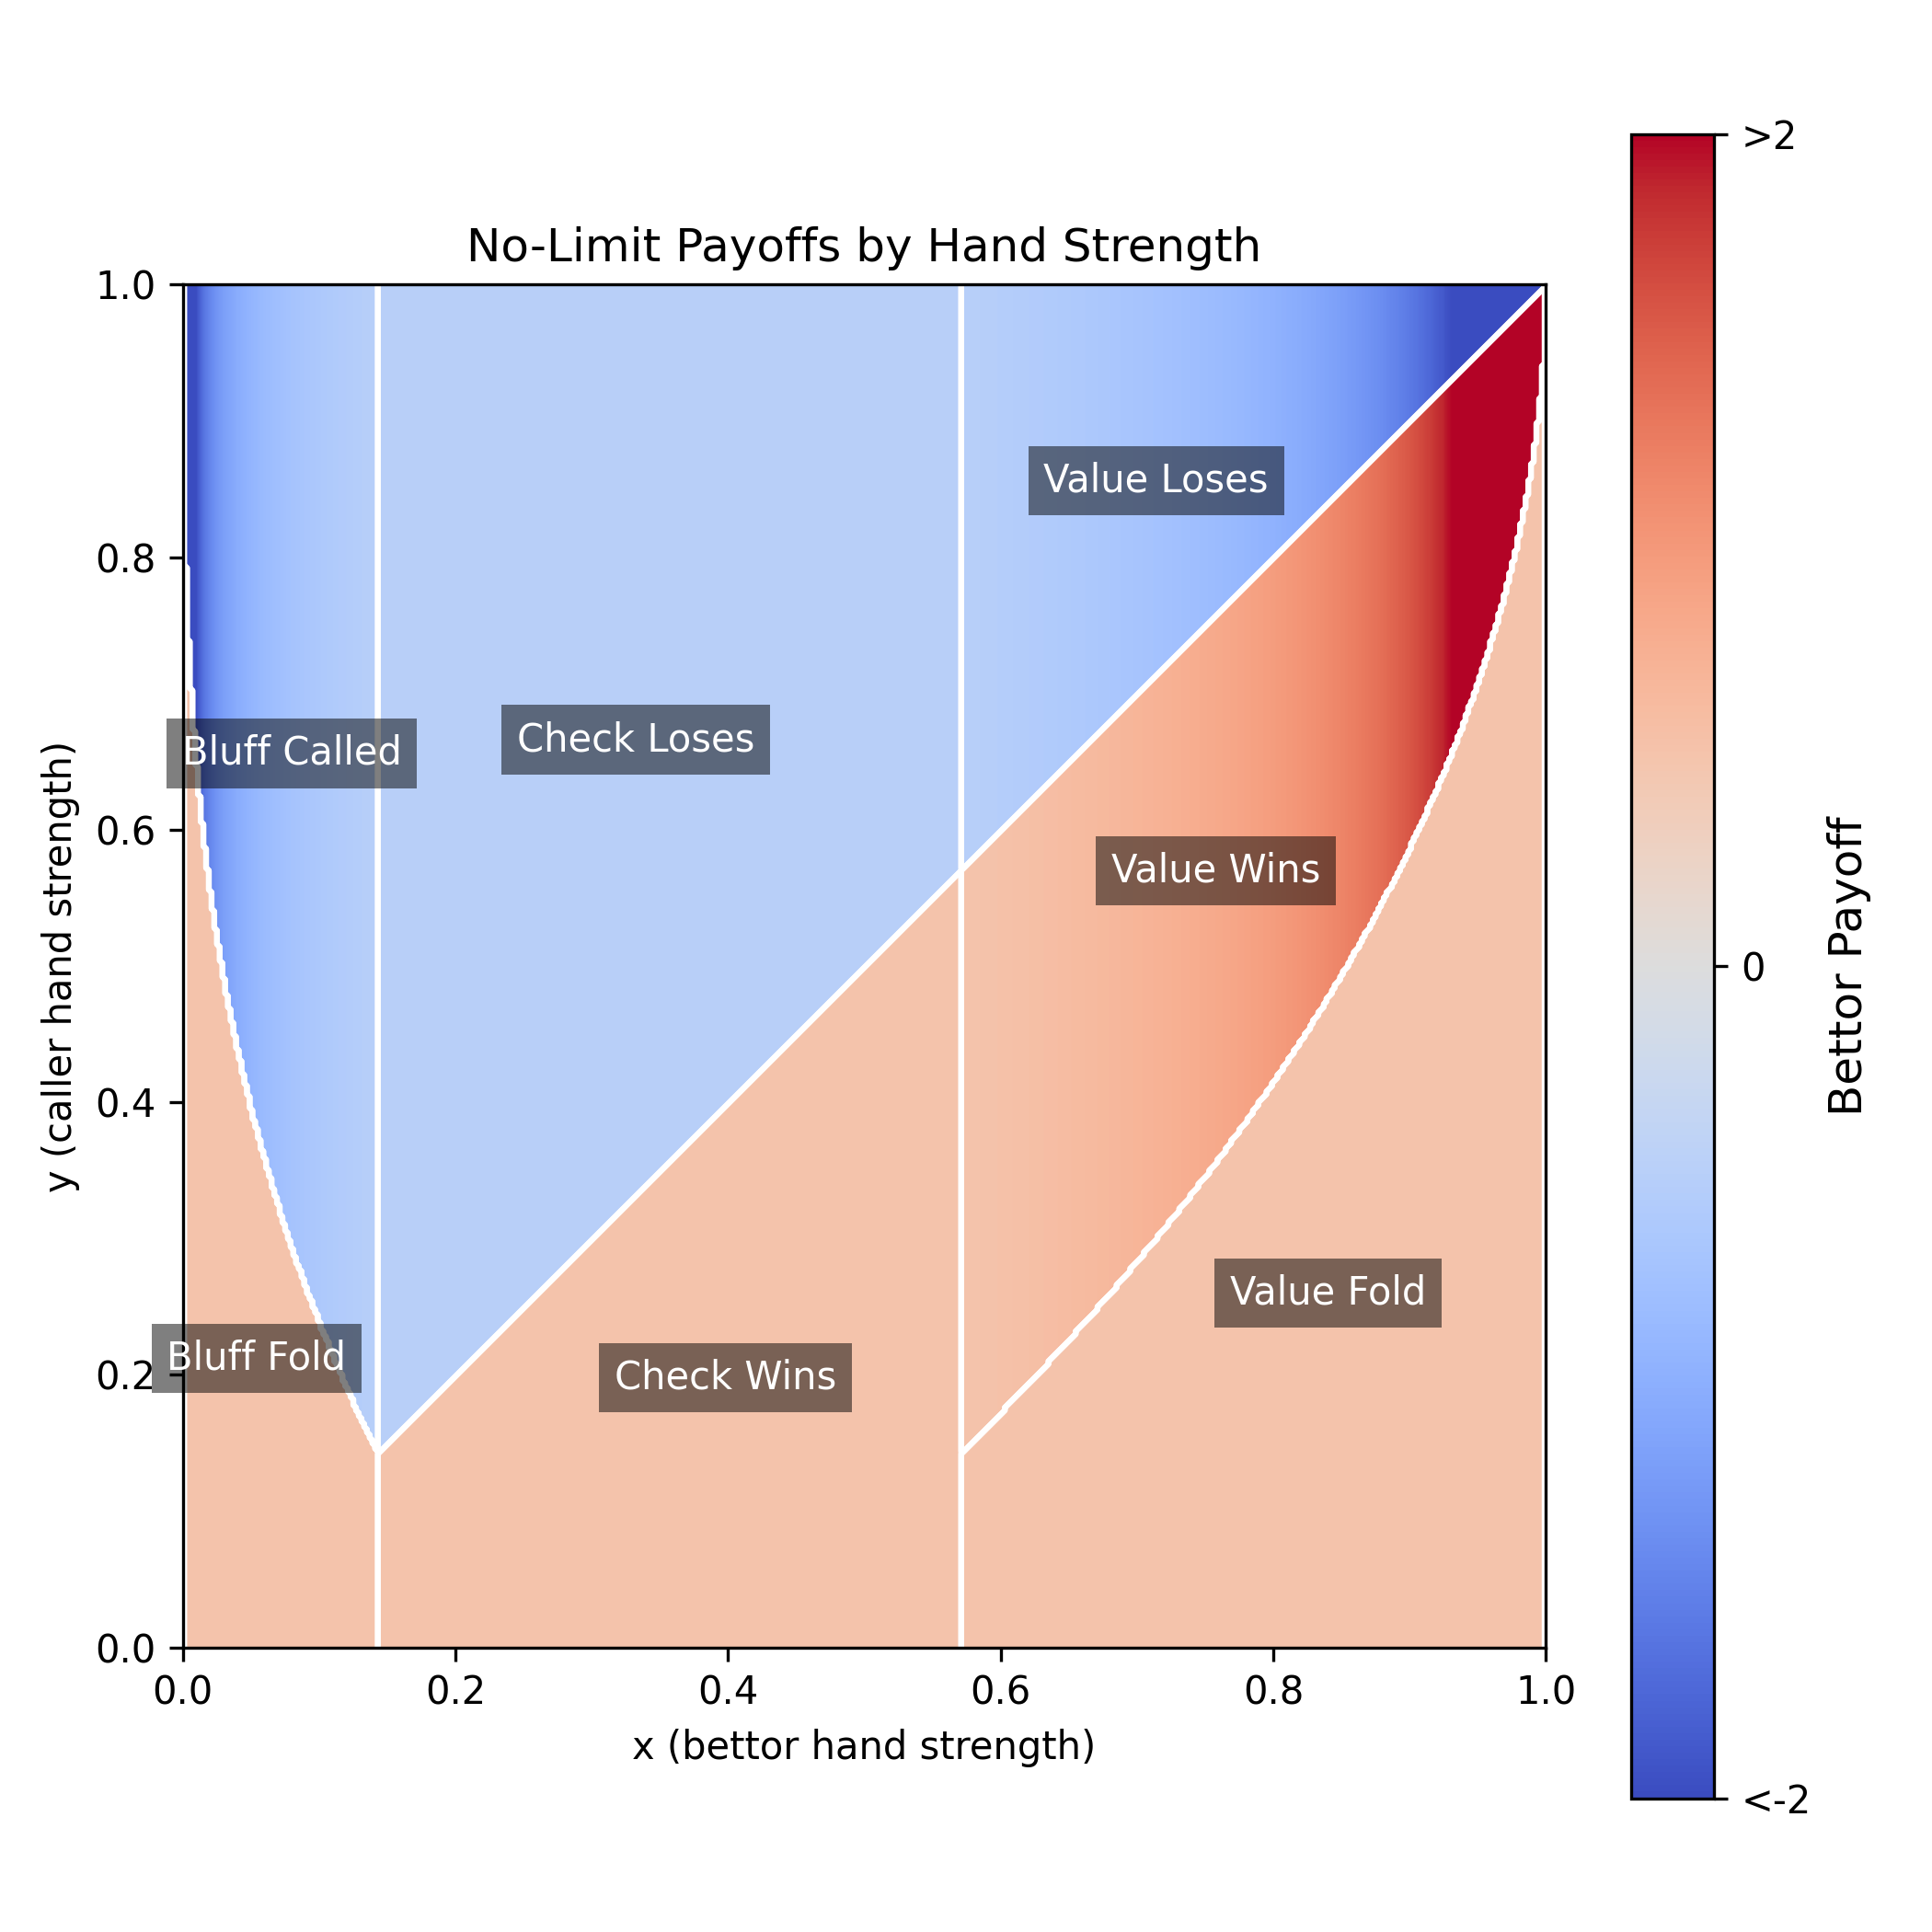
\includegraphics[width=\textwidth]{images/NoLimit_payoffs.png}
        \end{minipage}
    \end{adjustwidth}
    \caption{Bettor payoffs in Nash equilibrium as a function of hand strengths $x, y$ for fixed bet size $B=1$ (top left), and No-Limit Continuous Poker (bottom right). Intermediate plots show the payoffs for different values of $L$ and $U$ ranging from strict (fixed bet size $B=1$) to lenient (No limits). Regions are labeled according to the outcome of the game in Nash equilibrium.}
    \label{fig:payoffs}
\end{figure}

This visualization gives insight into exactly how the bettor is gaining value from the game. In line with experience of real poker, the biggest wins and losses occur when both hands are strong (top right of any plot), with the stronger of the two hands winning a large pot. However, we also see large payoffs when a very weak bettor bluffs big and gets called by a strong caller (top left). As the limits become more lenient, these cases become more extreme but also less likely, since making and calling maximum bets become more risky for both players. 

\subsection{Expected Value of Bettor's Hand Strengths}
\label{bettor_ev}

In addition to considering payoffs for a specific bettor-caller hand combination, we can also consider the expected value of given hand for the bettor, not knowing the hand of the caller. 

% x(2L + 1) - L(c[L] + 1) - 1/2 min value bet
% x(2U + 1) - U(c[U] + 1) - 1/2 max value bet
% x(2vinv[x] + 1) - vinv[x](c[vinv[x]] + 1) - 1/2 intermediate value bet
\begin{theorem}
    \label{thm:ev_bettor}
    Let $EV(x)$ denote the expected value of a value-betting hand $x$ in the unique admissible Nash equilibrium.
    \begin{equation}
        EV(x) = \begin{cases}
            x_2-\frac{1}{2} & \text{if } x \leq x_2 \\
            x-\frac{1}{2} & \text{if } x_2 < x \le x_3 \\
            x(2L + 1) - L(c(L) + 1) - \frac{1}{2} & \text{if } x_3 < x < v(L) \\
            x(2v^{-1}(x) + 1) - v^{-1}(x)(c(v^{-1}(x)) + 1) - \frac{1}{2} & \text{if } v(L) \leq x \leq v(U) \\
            x(2U + 1) - U(c(U) + 1) - \frac{1}{2} & \text{if } x > v(U)
        \end{cases}
    \end{equation}
\end{theorem}

\begin{customproof}
    For bluffing hands $x \leq x_2$, we can use a simple argument to show that the hand strength $x$ is actually irrelevant. The bettor never gets called by worse hands, so either the caller folds or calls with the best hand. In either case, the bettor's payoff has no dependence on $x$, so the payoff must be the same for all $x \leq x_2$ (otherwise, a the lower-payoff hands would imitate the strategy of the higher-payoff hands). We know that at $x=x_2$, the bettor is indifferent between bluffing and checking, so the payoff must be $x_2-\frac{1}{2}$ for all $x \leq x_2$.

    For checking hands $x_2 \leq x \leq x_3$, the bettor wins only the ante exactly when they have the best hand, which happens with probability $x$. The value of the ante is $\frac{1}{2}$, so the bettor's expected value is $x-\frac{1}{2}$.

    For any value betting hand, the bettor has three case to consider: the caller folds, the callers calls with a worse hand, or the caller calls with the best hand. We simply sum the expected value of each of these cases.

    \begin{align*}
        EV(x) & = \frac{1}{2} c(s) + (x - c(s)) \left(s+\frac{1}{2}\right) + (1-x) \left(-s-\frac{1}{2}\right)
    \end{align*}
    
    The last three cases come from substituting $L, v^{-1}(x), U$ for $s$ in the expression above and simplifying.
\end{customproof}

See figure \ref{fig:ev_x} for a visualization of this result.

\begin{figure}[h!]
    \centering
    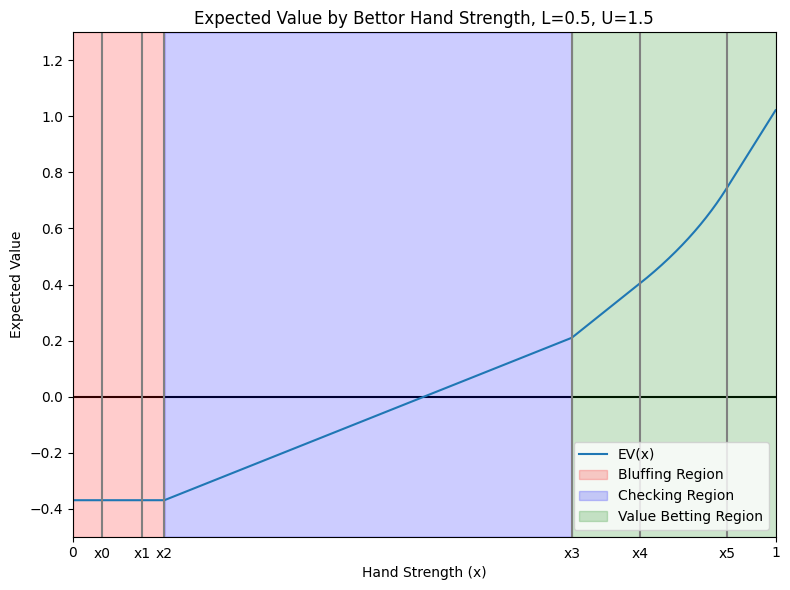
\includegraphics[width=\textwidth]{images/ExpectedPayoffs.png}
    \caption{Expected value of a value-betting hand $x$ in the unique admissible Nash equilibrium.}
    \label{fig:ev_x}
\end{figure}

We can quickly verify that the bettor's expected value is increasing in $x$. This must be the case, since with any given hand strength, the bettor can always choose to imitate the Nash equilibrium strategy of a weaker hand, so the stronger hand must be at least as good in expectation.

\begin{theorem}
    \label{thm:ev_increasing}
    For any fixed $L, U$, the bettor's expected value $EV(x)$ is increasing in $x$:

    $$ \frac{d}{dx} EV(x) > 0 $$
\end{theorem}

\begin{customproof}
    It is clear from inspection that any checking EV is higher than that of a bluff and that the checking EV is increasing in $x$. We also know that at $x=x_3$, the bettor is indifferent between checking and betting, so the EV of checking and betting must be equal at this point. Therefore, we only need to show that within the checking and value betting regions, the EV is increasing in $x$. This is obvious for checking hands. For value betting hands, we can take the derivative of the expression for $EV(x)$ with respect to $x$ and show that it is always positive. We consider the max and min betting hands first:
    
    \begin{align*}
        s = U \implies \frac{d}{dx} EV(x) & = 2U + 1 > 0  \\
        s = L \implies \frac{d}{dx} EV(x) & = 2L + 1 > 0 
    \end{align*}
    
    For intermediate value betting hands, we can use the chain rule to show that the EV is increasing in $x$:
    
    \begin{align*}
        \frac{d}{dx} EV(x) & = \frac{\partial EV(x)}{\partial x} + \frac{dEV(x)}{ds} \frac{d s}{d x} \\
    \end{align*}

    From the value optimality condition \ref{valueoptimality}, we know that $\frac{dEV(x)}{ds} = 0$ (otherwise, the bettor could gain value by varying the bet size). Clearly, $\frac{\partial EV(x)}{\partial x} > 0$.  Therefore, the derivative is positive, and the EV is increasing in $x$ for all value betting hands.
\end{customproof}

It is worth noting that the bettors strongest hands (right edge) actually seem to become less likely to make any profit more than the ante as limits increase. These strongest hands make very large bets, which force all but the strongest hands to fold, but win huge pots when they do get called. In more complicated poker variants, it is common to `slowplay' strong hands by checking or making small bets to induce bluffs from the opponent. In LCP, there is only one betting round and the caller is not allowed to raise, both of which make slowplaying obsolete. With extremely strong hands, the benefit of winning a large pot when betting big outweighs the lower likelihood of getting called.

We continue this analysis in the next section by considering how changing $U$ and $L$ affect various features of this equilibrium.
\end{document}